\documentclass[border=0pt]{standalone}
\usepackage[utf8]{inputenc}
\usepackage{graphicx}
\usepackage{subcaption}
\usepackage{tikz}
\usepackage{float}
\usepackage{natbib}
\usepackage[dvipsnames]{xcolor}
\usetikzlibrary{matrix, positioning,calc,arrows.meta, backgrounds,fit,shapes.geometric}
\tikzset{
    every node/.style={font=\small},
    greencycle/.style={fill=green!80!black!10,ellipse, align=center},
    rectred/.style={draw=red, fill=green!80!black!10, thick, rounded corners, align=center},
    rectblue/.style={draw=blue, rounded corners, align=center},
    yellowbox/.style={draw=black, fill=Dandelion, thick, rounded corners, align=center},
    bluecycle/.style={fill=NavyBlue, ellipse, align=center},
    arrow/.style={-{Latex[length=3mm]}, thick},
}

\begin{document}
\begin{minipage}{6.75in}
\centering
\captionsetup{type=figure}
\begin{subfigure}[b]{0.35\linewidth}\centering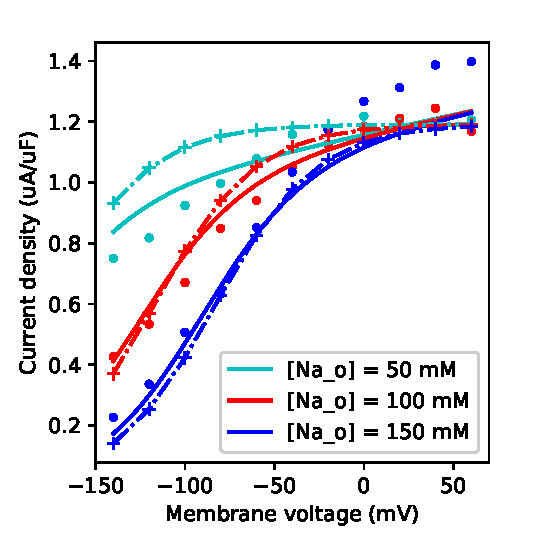
\includegraphics[width=\linewidth]{NKE_BG_6_stateV2_fig2b_fit.eps}\caption{Data from Figure 2b in (30)}\end{subfigure}
\begin{subfigure}[b]{0.35\linewidth}\centering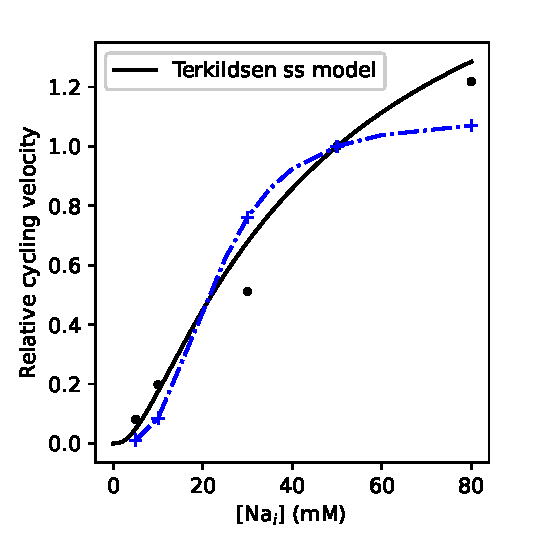
\includegraphics[width=\linewidth]{NKE_BG_6_stateV2_fig3a_fit.eps}\caption{Data from Figure 3a in (30)}\end{subfigure}
\begin{subfigure}[b]{0.35\linewidth}\centering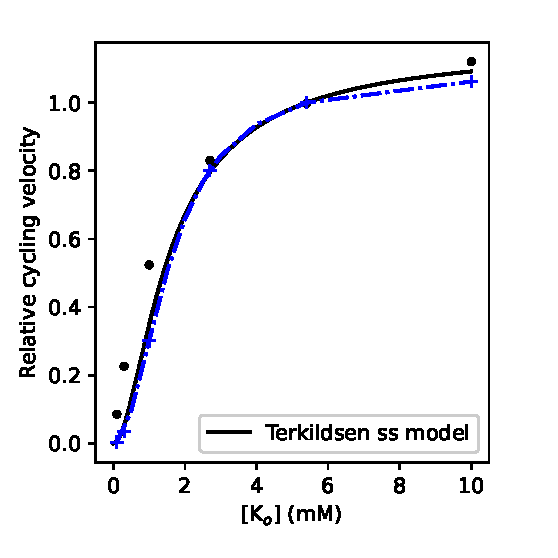
\includegraphics[width=\linewidth]{NKE_BG_6_stateV2_fig3b_fit.eps}\caption{Data from Figure 3b in (30)}\end{subfigure}
\begin{subfigure}[b]{0.35\linewidth}\centering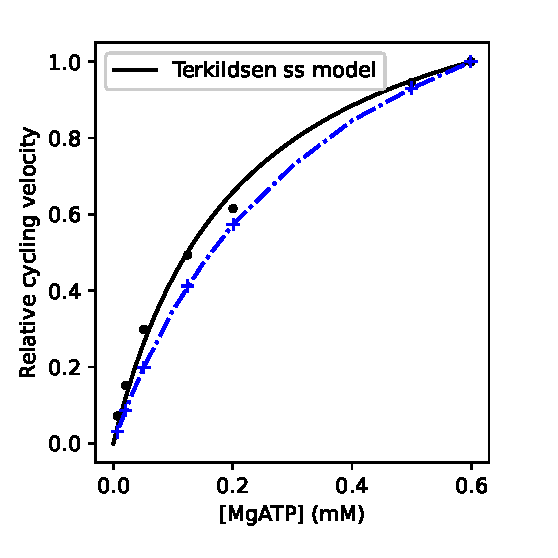
\includegraphics[width=\linewidth]{NKE_BG_6_stateV2_fig3c_fit.eps}\caption{Data from Figure 3c in (30)}\end{subfigure}
\end{minipage}

\end{document}
